\section[Ginzburg-Landau]{Ginzburg-Landau theory of superconductors}

We have seen how the appearance of $\bd \neq 0$ leads to superconductivity, i.e. the expectation value of the creation operator of a Copper-pair obtains a nonzero value. Let us formulate this in real space and define a wave-function $\psi(\bm{r}) $ for Cooper-pairs. This wave-function then describes a superconductor. It is a local field where $|\psi|^2$ describes the local density of Copper-pairs. We now set up an energy for the superconductor in terms of this field $\psi(\bm{r})$. Since this field has charge $e^* (e^* = 2e$, where $e =$ electron charge) this matter field $\psi$ must be minimally coupled to a gauge-field $\bm{A}$ (where the magnetic field $B_\mu = \ep_{\mu\nu\lambda} \partial_\nu A_\lambda$), and the magnetic field density is given by $B_\mu B_\mu = (\grad \cross \bm{A} )^2$.


\begin{equation}
\begin{aligned}
\Ha  &= \frac{\hbar^2}{2m} \left |\left (-i\grad - e^*\bm{A}\right )\psi \right |^2 + \alpha |\psi|^2 + \frac{u}{2} |\psi|^4 + \frac{1}{2}(\grad \cross \bm{A} )^2 \\
\psi &= |\psi| \e^{i\theta}
\label{Ham_ginz_lan}
\end{aligned}
\end{equation}

This is a phenomenological model of superconductivity written down long before the advent of the BCS-theory, and with very limited knowledge of what $\psi(\bm{r})$ actually represented! However, after the BCS-theory was formulated, L.P: Gorkov \emph{derived} the GL-theory from the BCS-theory, and it became clear that

\begin{equation}
\Delta (\bm{r}) = \mathcal{F}^{-1}(\Delta_k) \iff \psi(\bm{r}).
\label{gap_fourrier}
\end{equation}

$\langle \psi(\bm{r}) \rangle$ then serves as an order-parameter of the superconductor.

\begin{itemize}
\item 1. term in equation $\Ha$: Kinetic enegy
\item 2. term in equation $\Ha$: ``Chemical potential''-term for Cooper-pairs
\item 3. term in equation $\Ha$: Contact repulsion term between Cooper-pairs .
\item 4. term in equation $\Ha$: Magnetic field energy.
\end{itemize}
Note that
\begin{equation}
\begin{aligned}
\alpha =& \alpha(T) \\
=& \alpha_0 (T - T_C^{MF}), 
\label{alpha}
\end{aligned}
\end{equation}
where $T_C^{MF}$ is a mean-field critical temperature of a superconductor. $T < T_C^{MF} \implies \alpha<0$ , and thus the ``chemical potential''-term makes it energetically advantageous to allow non-zero Cooper-pair density $|\psi|^2$.

\textbf{Landau theory:} Ignore kinetic term 

\begin{equation}
\Ha_L = \alpha |\psi|^2 + \frac{u}{2} |\psi|^4.
\label{H_L}
\end{equation}

Determine $|\psi|$ by minimizing $\Ha$ with respect to $|\psi|$:
\begin{equation}
\frac{\dd{\Ha_L}}{\dd|\psi|} = 0
\end{equation}

\begin{equation}
\begin{aligned}
\frac{\dd{\Ha_L}}{\dd|\psi|}  =&  2\alpha |\psi| + 2u|\psi|^3 \\
=& |\psi| (2\alpha + 2u |\psi^2) \\
i)\;|\psi|  =& 0 \\
ii)\; |\psi|  =& \left ( - \frac{\alpha}{u}\right )^\frac{1}{2}  
\label{alpha}
\end{aligned}
\end{equation}
Knowing that $|\psi| $ is real and non-negative, it is clear that

\begin{itemize}
\item $\alpha>0$: Only one real solution, $|\psi| = 0 \implies \Ha_L = 0$ (minimum)
\item  $\alpha<0$: Two real solutions: 
\begin{itemize}
\item$|\psi| = 0 \implies \Ha_L = 0$ \
\item$|\psi| = \sqrt{\frac{|\alpha|}{u}} \implies \Ha_L = \alpha \frac{|\alpha|}{u} + \frac{u}{2} \frac{|\alpha|^2}{u^2}$
\item $\Ha^{Min}_L = - \frac{|\alpha|^2}{2u} < 0$
\end{itemize}
\end{itemize}

$|\psi| =   \sqrt{\frac{|\alpha|}{u}} $ gives a lower energy  than $|\psi| =0$ so $|\psi| =   \sqrt{\frac{|\alpha|}{u}} $ is the correct solution for $\alpha<0$. $\Ha_L^{min} = -\frac{|\alpha|^2}{2u}$. $\Ha$ as a function of $|\psi|$ is plotted in the figure below.


\begin{figure}
\centering
\subfloat{
    \centering
    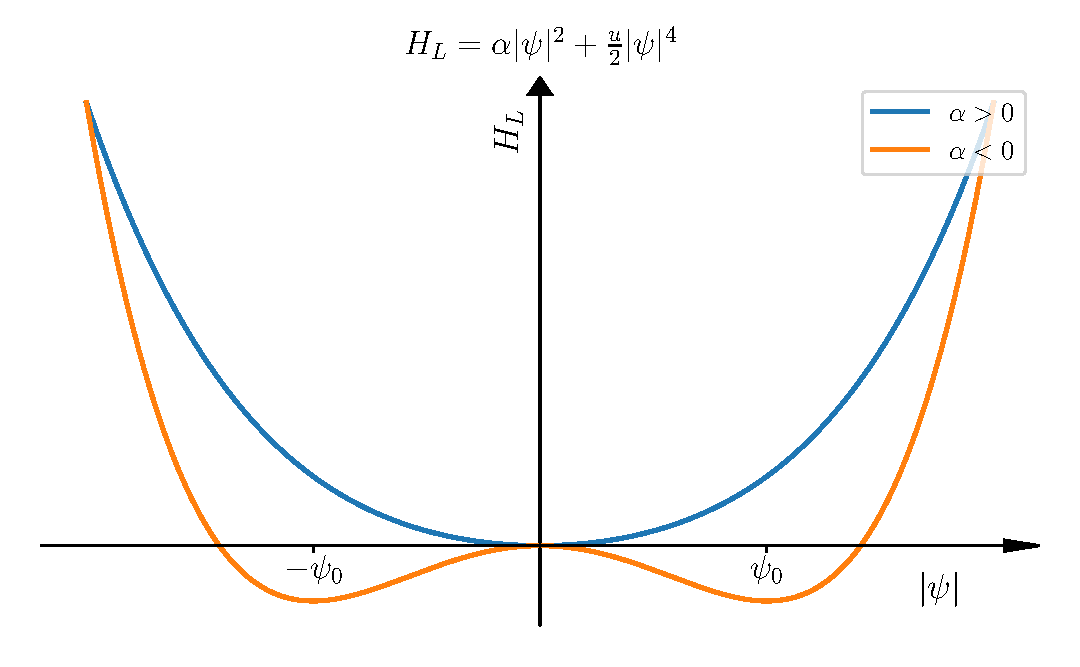
\includegraphics[width=\linewidth]{tex/pdf_files/H_L_1_D.pdf}
}
\caption{The Landau Hamiltonian, $\Ha_L$, as a function of $|\psi|$. Both signs of $\alpha$ are included, where $\alpha<0$, results in a minima in $\Ha_L$ at a nonzero $|\psi|$, denoted $\psi_0$.}
\label{fig:1D_H}
\end{figure}

For $\alpha<0$, we define 

\begin{equation}
\psi_0 = \sqrt{\frac{\alpha_0}{u}} (T_C^{MF} - T)^\frac{1}{2}.
\end{equation}

Observe that the critical exponent $\beta = \frac{1}{2}$ and that $\psi_0$ is a real number for $\alpha<0$, i.e. at $T<T_C^{MF}$. 


\newpage

Even though $\Ha_L$ only depends on the modulus of $\psi$, $\psi$ is still a complex number that can be written on the form $\psi=|\psi| \e^{i\theta}$. So we have the  energy landscape in the complex $\psi$-space as illustrated in the figure above.
\begin{figure}
\centering
\subfloat{
    \centering
    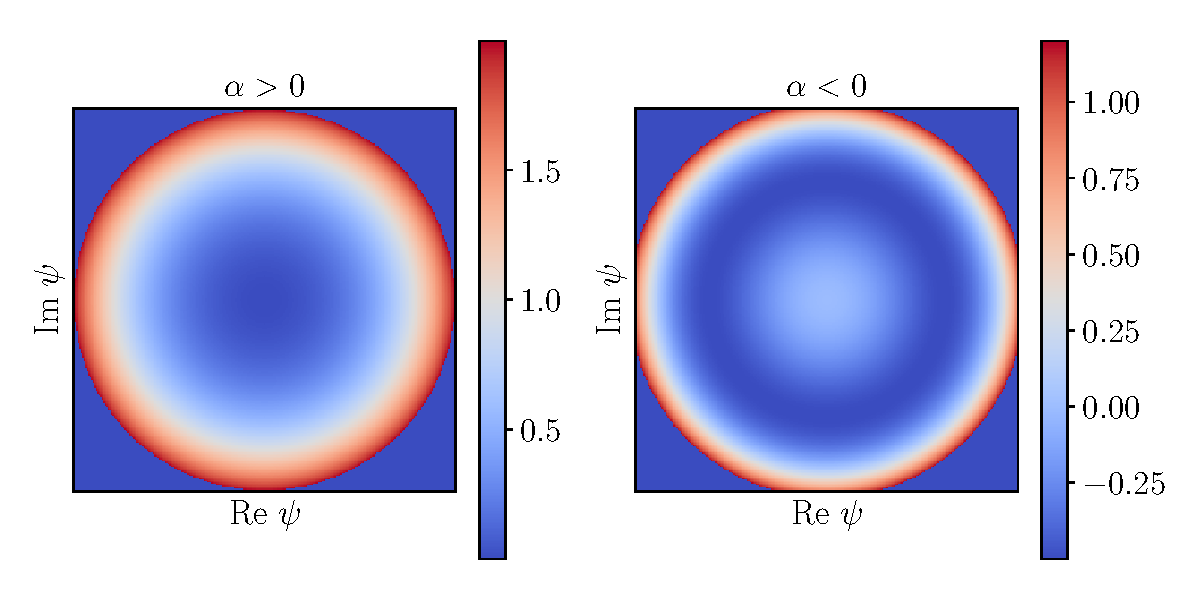
\includegraphics[width=\linewidth]{tex/pdf_files/H_L_2_D.pdf}
}
\caption{The Landau Hamiltonian, $\Ha_L$, as a function of the complex variable $\psi$. For $\alpha>0$ it is a simple paraboloid, monototonically increasing as the modulus of $\psi$ increases. However for $\alpha<0$, there exists a nonzero value of $|\psi|$ that yields a minima for $\Ha_L$.  It results in a Hamiltonian that bears a resemblence to a ''Sombrero hat''. Note that the minimum is only unique for the modulus, there is still a massively degenerate $\Ha_L$-minimum if the phase is included.}
\label{fig:1D_H}
\end{figure}

Note that from the ``Sombrero-hat''-picture, fluctuations in $\theta$ cost no energy in Landau-theory. On the other hand we see that fluctuations in $|\psi|$ around $\psi_0$ \emph{do} cost energy. 


Phase-fluctuations are ``massless''. Amplitude-fluctuations are ``massive''. 

Consider now also the kinetic energy and allow for phase-fluctuations and amplitude fluctuations. In other words, we allow 

\begin{equation}
\begin{aligned}
\psi =& (\psi_0 + \psi_1) \e^{i\theta}\\
\psi_0 =& \sqrt{\frac{|\alpha|}{u}} \; ; \; \psi_1 \; \mathrm{real}.
\label{psi_fluc}
\end{aligned}
\end{equation}


Consider first the Landau terms 

\begin{equation}
V(|\psi|) = \alpha |\psi|^2 + \frac{u}{2} |\psi|^4.
\label{V_psi}
\end{equation}

Expanding equation \cref{psi_fluc} to second order in $\psi_1$ for $\alpha<0$ yields


\begin{equation}
\begin{aligned}
V(|\psi|) & \\
=& \alpha (\psi_0^2 + 2\psi_0 \psi_1 + \psi_1^2) \\
+& \frac{u}{2} (\psi_0^4  \ 4\psi_0^3 \psi_1 + 6 \psi_0^2 \psi_1^2 + \mathcal{O}(\psi_1^3)) \\
=& \alpha_0 \psi_0^2 + \frac{u}{2} \psi_0^4 + 3u\psi_0^2\psi_1^2 + \alpha \psi_1^2 + \psi_1(2\alpha\psi_0 + 2u\psi_0^3), \mathrm{last}  \; \mathrm{term} = 0 \\
=& -\frac{\alpha^2}{2u} + \psi_1^2(\alpha - 3\alpha) \\
=& -\frac{\alpha^2}{2u} + 2|\alpha| \psi_1^2 \\
=& \Ha_L^{min} + 2\alpha \psi_1^2.
\label{psi_fluc_expansion}
\end{aligned}
\end{equation}

Consider next the kinetic energy term $\frac{\hbar^2}{2m} \left |\left (\frac{\grad}{i} - e^*\bm{A}\right )\psi \right |^2$

\begin{equation}
\begin{aligned}
& \left (-i\grad - e^*\bm{A}\right )(\psi_0 + \psi_1) \e^{i\theta} \\
=& -i\grad\psi_1  \e^{i\theta} - e^* \bm{A} \psi_1  \e^{i\theta} \\
+& (\grad \theta - e^* \bm{A} )(\psi_0 + \psi_1)  \e^{i\theta} \\
\simeq&  \left (-i\grad\psi_1 + (\grad \theta - e^* \bm{A} ) \psi_0 \right ) \e^{i\theta}.
\label{psi_fluc_expansion_kin}
\end{aligned}
\end{equation}
Here we have kept only terms that are linear in the fluctuations fields $\psi_1, \theta, \bm{A}$, since we will square the above expression to get the kinetic energy. 

\begin{equation}
\begin{aligned}
&\frac{\hbar^2}{2m} \left |\left (-i\grad - e^*\bm{A}\right )\psi \right |^2 \\
=& \frac{\hbar^2}{2m} \left [ (\grad \theta - e^* \bm{A} )^2 \psi_0^2 + (\grad \psi_1)^2 \right ]. \\
\Ha =& \Ha_L^{min} + \frac{\hbar^2 \psi_0^2}{2m} (\grad \theta - e^* \bm{A} )^2 \\
 +& \frac{\hbar^2}{2m} (\grad \psi_1)^2 + 2|\alpha| \psi_1^2 + + \frac{1}{2}({\grad} \cross \bm{A} )^2.
\label{H_fluc}
\end{aligned}
\end{equation}

When $\alpha<0$, we see that amplitude-fluctuations $\psi_1$ are always massive, even if we make $\grad \psi_1$ arbitrarly small. Fluctuations in the phase $\theta$, on the other hand are massless, which means they are much easier to excite, and can be made to have arbitrarly low energy by making $\grad \theta$ arbitrarly small. The same is true for the $(\grad \cross \bm{A})^2$-term. We therefore focus on the fluctuations in $\theta$ and $\bm{A}$, and discard the $\psi_1$-part.  Also discarding $\Ha_L^{min}$ and introducing 

\begin{equation}
\rho_s \equiv \frac{\hbar^2 \psi_0^2}{m},
\end{equation}

we have 

\begin{equation}
\Ha = \frac{\rho_s}{2}  (\grad \theta - e^* \bm{A} )^2 + \frac{1}{2}({\grad} \cross \bm{A} )^2.
\label{Ham_rel_fluc} 
\end{equation}

This is the theory descrbing the relevant fluctuations around the Landau mean-field theory.

By introducing the current 



\begin{equation}
\begin{aligned}
\bm{j} =& - \frac{\partial \Ha}{\partial (e^* \bm{A})} \\
=& \rho_s (\grad \theta - e^*\bm{A}),
\end{aligned}
\end{equation}

we can describe the current in the superconducting state with phase-ordering as 

\begin{equation}
\bm{j}  = -e^* \rho_s \bm{A}.
\label{j_super} 
\end{equation}

Equation \cref{j_super} is exactly the consitutive relation for $\bm{j}$ that we used in combination with Maxwell's equations to give the Meissner-effect.

Note that the theory has a local $U(1)$ gauge-invariance, $e^*\bm{A}' =  e^*\bm{A} - \grad \theta$. This transformation leaves $\Ha$ in equation \cref{Ham_rel_fluc} invariant

\begin{equation}
\Ha = \frac{\rho_s}{2} e^{*^2} {\bm{A}'}^2 + \frac{1}{2}({\grad} \cross \bm{A}')^2.
\label{Ham_rel_fluc_inv} 
\end{equation}

Note that it now appears that the gauge-field (photon) has acquired a mass 
\begin{equation}
m_A^2 \equiv  e^{*^2} \rho_s.
\end{equation}

Also note that we \emph{used} the $U(1)$ gauge-invariance to arrive at this conclusion. We thus have 

\begin{tcolorbox}
\begin{equation*}
\rho_s \neq 0 \iff \psi_0 \neq 0 \iff \mathrm{Cooper-pairs}.
\end{equation*}
\end{tcolorbox}

$\psi_0$ plays the role of a Higgs-field, and the presence of a Higgs condensate (in this case, a superconductor) gives the photon a \emph{mass $m_A$}. This leads to the Meissner-effect. 

The Ginzburg-Landau theory for a superconductor is identical in form to the Higgs-sector of the Standard model. 


\begin{tcolorbox}
The Bogoliubov quasiparticles described by $\eta_k$ and $\gamma_k$ in the BCS-theory are fermionic analogs of the so-called Higgs-particle. 
\end{tcolorbox}

